\documentclass{article}
\usepackage[utf8]{inputenc}
\usepackage{graphicx}
\usepackage{amsmath}
\usepackage[section]{placeins}
\usepackage{wrapfig}
\usepackage{tikz}
\usepackage{lipsum}
\usepackage[utf8]{inputenc}
\usepackage{amsmath}
\usepackage{caption}
\usepackage[margin = 1in]{geometry}
\usepackage[backend=biber]{biblatex}
\addbibresource{sources.bib}
\bibliography{sources.bib}
\usepackage{hyperref}
\usepackage{float}
\usepackage{graphicx}
\usepackage{hyperref}
\usepackage{makecell}
\usepackage{textcomp}
\usepackage{gensymb}
\usepackage{xcolor}
\usepackage{fancyhdr}
\usepackage{lipsum}
\usepackage{pdfpages}
\usepackage{wrapfig}
\usepackage{subcaption}
\usepackage{setspace}
\usepackage{nomencl}
\usepackage{listings}
\usepackage{hyperref}
\usepackage{multicol}
\bibliography{sources}
 \usepackage{float}


\title{Titan Aircraft Design}
%\author{Annie Price}
%\date{June 2021}

\begin{document}

\maketitle

\section{Introduction and Mission Requirements}
\label{sec:Titan Aircraft Design}

In this section, the Titan Aircraft sizing and performance analysis in NASA's OpenVSP is presented. 

\subsection{Mission Requirements}
\label{sec:Mission Requirements}

The design of the Titan Aircraft was driven by the key mission requirements. The mission requirements for the aircraft are presented in the following table:

\begin{table}[H]
\centering
\begin{tabular}{|c|c|} 
\textbf{Requirement} & \textbf{Value} \\
\hline 
\hline
    Range & Infinite \\
\hline 
    Maximum Cruise Speed & 266 m/s\\
\hline 
    Takeoff Distance & 500m\\
\hline 
    Cruise Altitude & 1km\\
    \end{tabular}
    \caption[Table] {Table Summarizing the Mission Requirements for the Titan Aircraft}
\label{tab:parameters}
\end{table}


In addition to these mission requirements, certain assumptions about the aircraft were made. First, the aircraft design needed to allow for hypersonic entry into Titan's atmosphere. The assumption was made that there is constant electric power of up to 1MW coming from the fusion reactor during all stages of flight. Another key assumption was that the aircraft never loses any mass due to fuel burn. This means there was no need for any initial weight fraction calculations, since it was assumed the dry mass of the aircraft will be 2000kg for all stages of flight. The mass of the engine was assumed to be a constant 1000kg. 

\subsection{Initial Sizing}
\label{sec:initial sizing}

Before any sketching of the aircraft could occur, initial conceptual sizing was necessary in order to make sure a design that met all of the mission requirements was feasible. As stated above, there was no need to go through calculations for a takeoff weight buildup or estimate fuel fractions for different stages of flight, since the aircraft weight would always remain a constant 2000kg due to the fusion reactor's constant electric power source. Therefore, the take-off weight calculation was unnecessary, and it was possible to go right to airfoil and geometry selections. 

\subsection{Wing Loading and Geometry Selection} 
\label{sec: Wing Loading and Geometry Selection} 

The airfoil selection is incredibly important to the lift and drag of the aircraft. A symmetric wedge shape was chosen for the initial design, since the aircraft will be subjected to supersonic flow when entering Titan's atmosphere. 


Next, power-to-weight ratio and wing loading needed to be calculated. The power-to-weight ratio is used to describe a propeller powered aircraft and is the equivalent to the "thrust-to-weight" term for a jet engine aircraft [1]. Since this aircraft is driven by ducted fans when in transonic flow in Titan's atmosphere, the power-to-weight ratio is needed.  A critical parameter in wing loading is the stall speed. The stall speed of the aircraft is directly determined by the wing loading and the maximum lift coefficient and is critical to flight safety [1]. The approach speed, which is also used to determine takeoff length, is defined by the stall speed [1]. The FAA defines acceptable stall speeds for different type of aircraft based on applications [2]. Since the coefficient of gravity on Titan is around 7.3 times weaker than on Earth, the stall speed is going to be much lower for an aircraft on Titan. Given the gravity constant on Titan is 
\begin{equation} 
1.352 m/s^{s}
\end {equation}

as well as the required takeoff field length of 500m, kinematic equations were used to estimate the stall speed[1]: 

\begin{equation}
s_{takeoff} = 1/2*a*t^{2} 
 \label{eq: kinematic distance}
\end {equation} 

\begin{equation}
    t = (\frac{s_{takeoff}*2}{a})^{1/2} = (\frac{500m*2}{1.352m/s^{2}})^{1/2} = 27.196 s
    \label{eq: kinematic time}
\end{equation}

\begin{equation} 
v_{final} = v_{initial} + a*t = 1.352m/s^{2} * 27.196s = 36.7696 m/s = v_{takeoff}
\label{eq: kinematic speed}
\end{equation}

The stall velocity is dependent upon the takeoff speed and is given through the following formula[1]: 

\begin{equation} 
v_{stall} = \frac{v_{takeoff}}{1.2} = 30.641 m/s
\end{equation}

The stall speed adds a vertical line to the thrust loading vs wing loading graph and acts as the maximum limit for W/S. The design must be to the left of this vertical line. 
Given this estimate of stall speed, the wing loading could be estimated. The wing loading is given by the follow equation[1]: 

\begin{equation}
    V_{stall} = (\frac{W}{S}*\frac{rho}{C_{l_{max}}})^{1/2}
\end{equation}

 $({C_{l_{max}}})$ was estimated as 3.0 for STOL aircraft.
 
 Given the above parameters, the maximum wing loading was found with the following formula[1]: 
 
 \begin{equation} 
 \frac{W}{S} = (V_{stall}*C_{l_{max}}/rho)^{1/2} = 27.0849
 \end {equation} 
 
 This is the vertical line on the thrust-to-weight vs. wing loading graph, which provides a design constraint for the aircraft. 
 
 The power-to-weight vs. wing loading graph for different stages of flight was then generated in Matlab, which provides key design points from which the aircraft may be sketched. The constant weight of the aircraft will drastically impact the power-to-weight vs. wing loading graph and design point chosen. All equations from this graph come from the master equation[2]: 
 
 \begin{equation}
     \frac{T_{s.l.}}{W_{to}} = \frac{\beta}{\alpha}* (\frac{q_{\inf}*S}{\beta*W_{TO}}*(K_{1}*(\frac{n*\beta*W_{to}}{q_{\inf}*S})^{2} + K_{2}*(\frac{n*\beta*W_{to}}{q_{\inf}*S}) + C_{D_{0}} + C_{D_{R}}) + \frac{P_{s}}{V})
 \end{equation}
 

 First, the thrust-to-weight ratios were found. The thrust-to-weight ratio at cruise represents the amount of thrust needed to maintain the cruise velocity of 100m/s. The equation for thrust loading during cruise is given by the following equation[1]: 
 
 \begin {equation} 
 \frac{T_{cruise}}{W_{takeoff}} = \frac{q_{cruise}*C_{d_{0}}}{W/S} + k*(\frac{W/S}{q-C_{l_{0}}})
 \end {equation} 
 
 The thrust-to-weight ratio during takeoff is dependent on the thrust-to-weight ratio during cruise[1]: 
 
 \begin{equation}
      \frac{T_{takeoff}}{W_{takeoff}} =  \frac{T_{cruise}}{W_{takeoff}} * \frac{W_{cruise}}{W_{takeoff}}*\frac{T_{takeoff}}{T_{cruise}} =  \frac{T_{cruise}}{W_{takeoff}} * 1 * \frac{T_{takeoff}}{T_{cruise}}
 \end{equation}
 
 Finally, the thrust-to-weight ratio during climb is given by[1]: 
 
 \begin{equation} 
\frac{T_{climb}}{W_{takeoff}} = \frac{q_{climb}*C_{d_{0}}}{W/S} + k*(\frac{W}{S}*\frac{n}{q_{climb}*\pi*AR*\epsilon})
 \end{equation}
 
 The relation between the thrust-to-weight ratio and the power-to-weight ratio is given by the following formula[1]: 
 
 \begin{equation}
 \frac{T}{W} = \frac{500*\eta_{prop}}{V}*\frac{hp}{W}
 \end{equation}
 
 
 where $\eta_{prop}$ is the efficiency of the propellers, calculated in the next section, and hp is the horsepower of the aircraft. The thrust-to-weight ratios were calculated for the takeoff, climb, and cruise segments and then were converted to power-to-weight terms using the above equation before being plotted in matlab as functions of wing loading for different values of wing loading, varying from 1 to 50.
 

 
 
 The final power-to-weight vs. wing loading graph is shown below: 
 
 \begin{figure}[H]
 \centering
    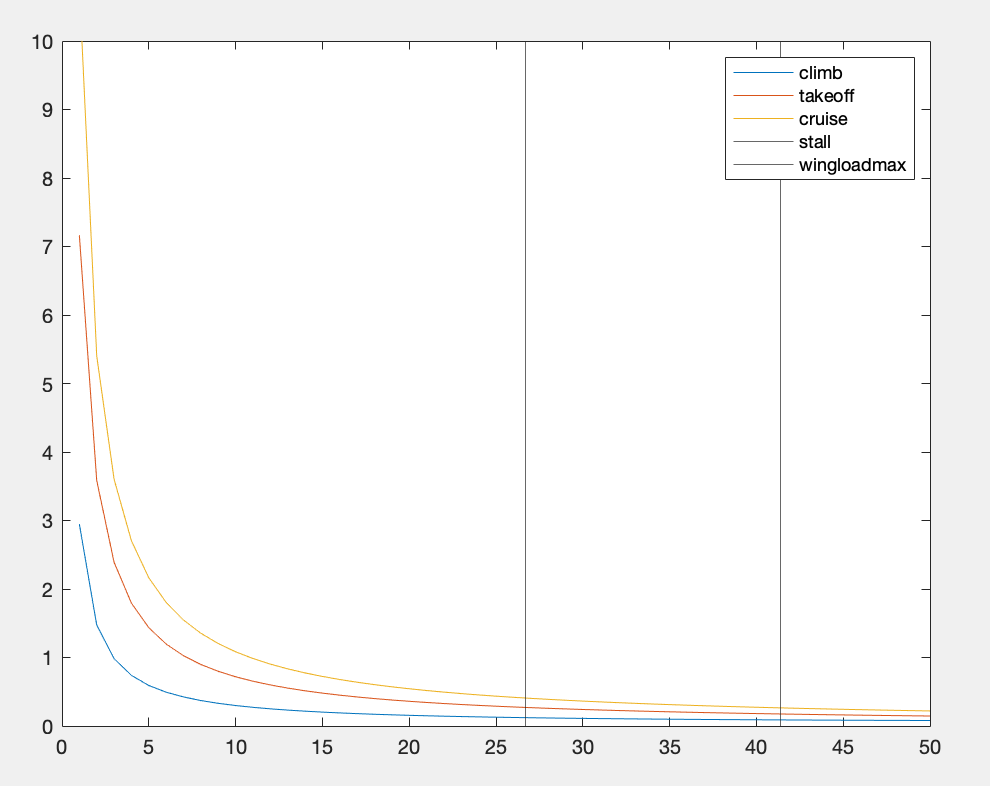
\includegraphics[width=0.90\textwidth]{Figures/Powerload.png}
    \caption[Power-to-Weight vs. Wing Loading MATLAB Plot]{Power-to-Weight vs. Wing Loading MATLAB Plot. \label{fig:Powerloading} }
 \end{figure}
 
 

The power-to-weight vs. wing loading graph allows selection of a design pint for the aircraft. Since the wing loading for stall is at 27.0849, the  design must be to the left of this curve. The design point must also be above the cruise and climb curves on the graph for a T/W vs. W/S. Climb is the lowest curve, so the design point must be above that curve. A wing loading value of 25 was chosen. From this W/S value, the initial wing geometry was calculated, beginning with the wing area (S): 

\begin{equation}
    \frac{W}{S} = 25
    2704 = 25*S
\end{equation}

The wing area, S, was found to be 108.16 ${m^{2}}$. Converting this to ${ft^{2}}$, which is the default unit value in OpenVSP gives a value of 1164.22455 ${ft^{2}}$. 

Next, the wing span can be found given the formula[1]: 
\begin{equation}
b = (A*S)^{1/2}
\end{equation}
where "A" refers to the aspect ratio, estimated from the initial engine data to be 1.7. Therefore, b = 44.487 ${ft}$. 
Next, the root chord was estimated through the following formula[1]: 
\begin{equation}
C_{root} = \frac{2*S}{b(1 + \lambda)}
\end{equation}
where ${(\lambda)}$ is the taper ratio, the ratio between the tip chord and the center line root chord. Since the wing will be a delta wing and will have a high sweep, the taper ratio is estimated for now to be 0.25. Therefore, $C_{root}$ is estimated as 41.87. 
The tip chord is simply the product of the taper ratio and the root chord[1]: 
\begin{equation} 
C_{tip} = {\lambda}*C_{root}
C_{tip} = 0.25 * 41.87 = 10.47
\end{equation}
The mean aerodynamic chord can be estimated as[1]: 
\begin{equation}
C_{mean} = \frac{2}{3}*C_{root}*\frac{1+\lambda+(\lambda)^2}{1+\lambda} = 29.309
\end{equation}
Finally, the span-wise mean aerodynamic chord's location from the center line for a wing or a tail is given by[1]: 
\begin {equation}
Y_{bar} = \frac{b}{6}*\frac{1+2*\lambda}{1+\lambda} = 232.84 ft. 
\end{equation}



%\subsection{Flight Envelope}
%The aircraft's flight envelope demonstrates the static and dynamic 
%conditions within which the aircraft can operate. A mesh grid of altitude versus airspeed was plotted for values ranging from 0-1000km and 0-1000 km/s. Specific excess power curves were then plotted

\section{OpenVSP Sketching and Analysis}
\label{sec:OpenVSP Sketching and Analysis}
After setting initial parameters for the main wing geometry, the first iteration of the aircraft was sketched in NASA's Open Vehicle Sketch Pad. A delta-winged aircraft was chosen due to the hypersonic re-entry mission requirement. A double wedged airfoil is commonly used in supersonic applications, so it was chosen for the first iteration. Wedged airfoils have sharp leading edges in order to reduce wave drag [3]. Wave drag in supersonic flight is caused by the formation of normal shock waves in supersonic flow that detach from the leading edge of the wing[3]. Having a blunt leading edged airfoil increases this drag, but having a sharp leading edged airfoil allows oblique shock waves to attach to the leading edge and decreases the area of high pressure ahead of the wing, therefore reducing wave drag [3]. Two ducted fans were added near the back of the fuselage in order to take advantage of Boundary Layer Ingestion. Boundary Layer Ingestion involves the placement of electric propulsors like ducted fans, rotors, or propellers, so that they ingest the fuselage boundary layer flow near the tail end of the fuselage [6]. Boundary Layer Ingestion systems increase propulsive efficiency by reducing drag and can be implemented on the hybrid wing body[6], which is the configuration of this aircraft. The ducted fans are both connected in parallel to the fusion reactor main engine, so it is assumed that there is constant power across the both of them. The first sketch of the aircraft is shown below: 

\begin{figure}[H]
    \centering
    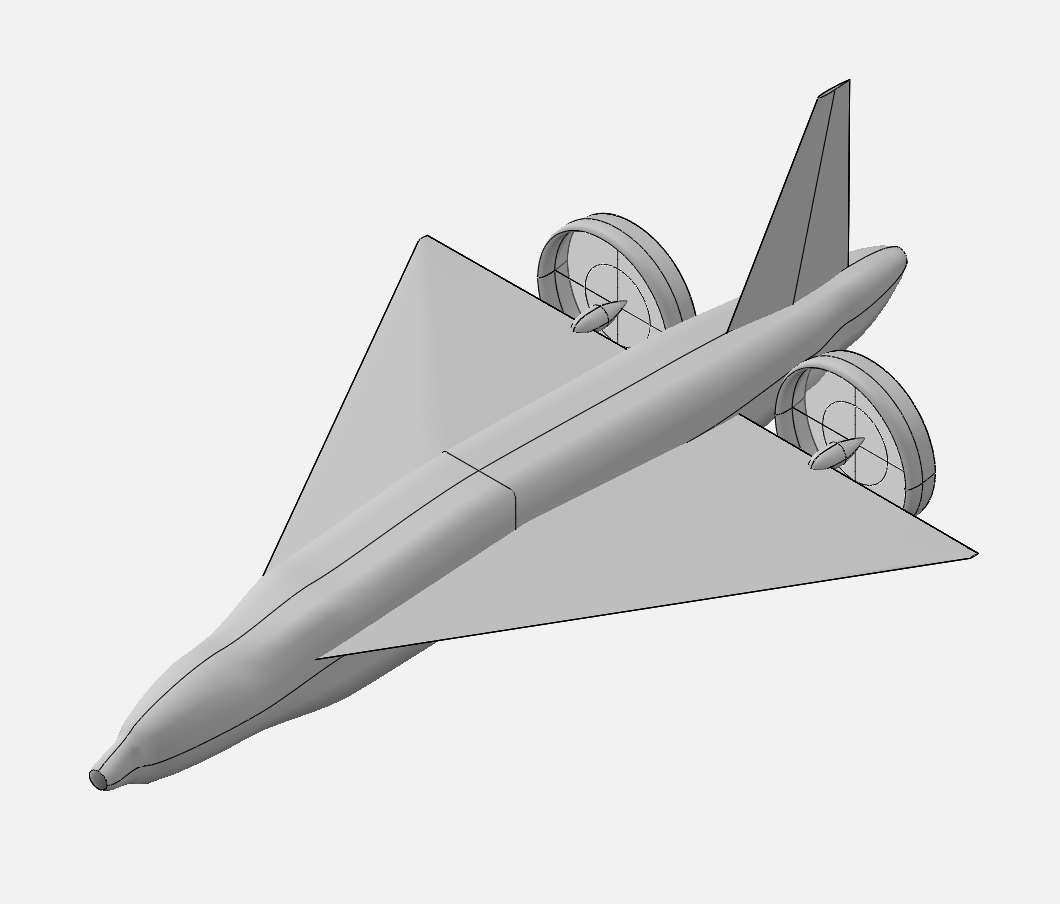
\includegraphics[width=0.90\textwidth]{Figures/TitanLanderInitialIsoView.png}
    \caption[First Iteration of the Titan Aircraft, with a Hybrid Delta-Winged Body, Two Ducted Fans at the Rear End of the Fuselage]{First Iteration of the Titan Aircraft, with a Hybrid Delta-Winged Body, with Two Ducted Fans at the Rear End of the Fuselage. \label{fig:TitanLanderv1} }
\end{figure} 


The ducted fans are modeled as actuator disks in this model. A simple vertical stabilizer with a double wedged arifoil was chosen. This configuration was then analyzed using the VSPAero vortex lattice solver. The aircraft was first analyzed in transonic flow only, since this is the flow condition during cruise. Therefore, Mach number was set to 0.85. L/D was analyzed for varying angles of attack from 1-15. The analysis results are shown below: 

\begin{figure}[H]
    \centering
    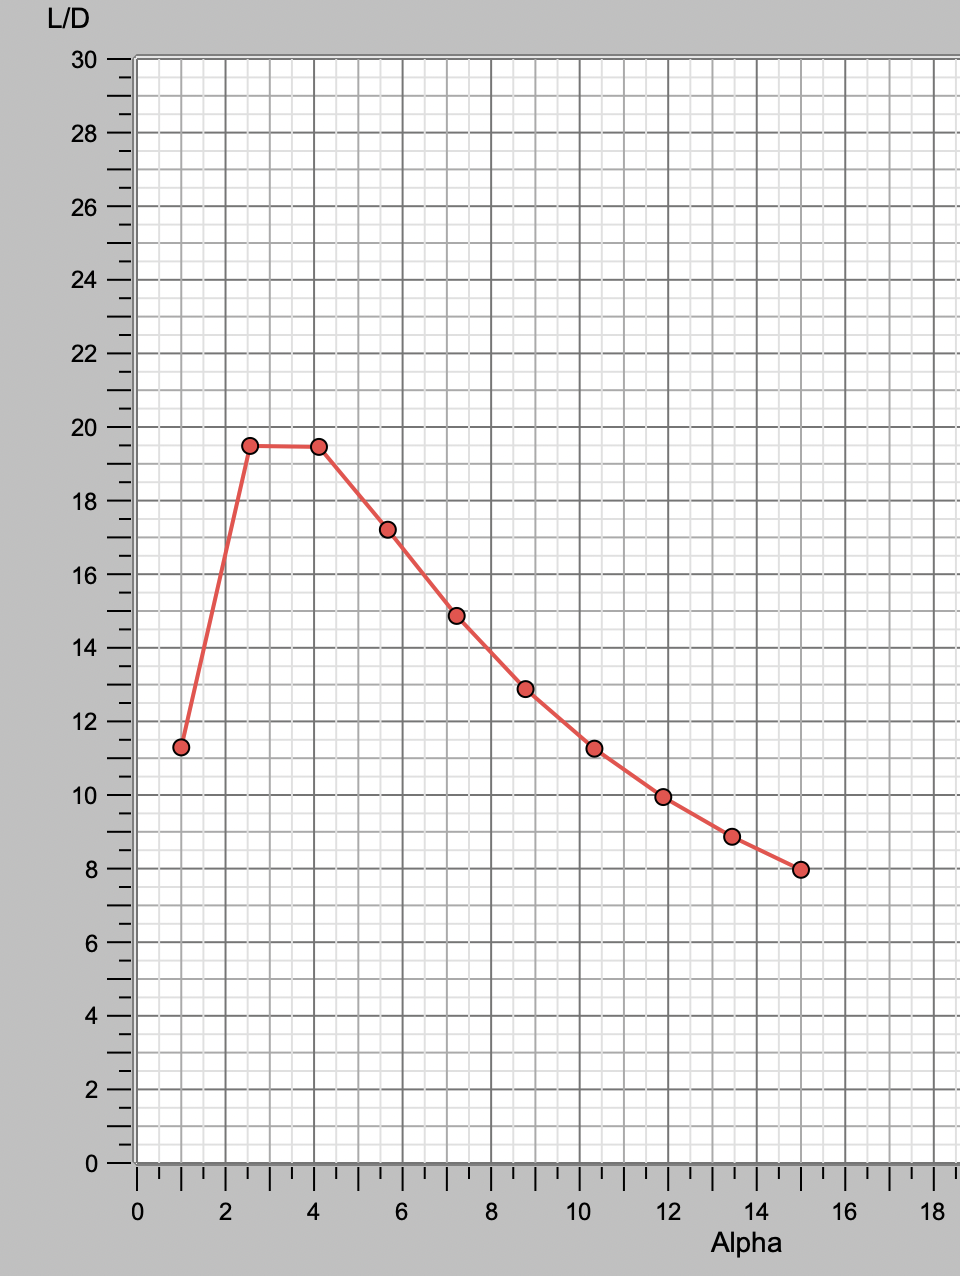
\includegraphics[width=0.90\textwidth]{Figures/VSP_Initial.png}
    \caption[L/D vs. Angle of Attack for the Initial Aircraft Design]{L/D vs. Angle of Attack for the Initial Aircraft Design. \label{fig:LDInitial} }
\end{figure} 
    
At an angle of attack of 3, the L/D ratio is 19.5, which is more than the assumed L/D in the thrust-to-weight vs. wing loading matlab code (L/D at cruise was assumed to be 18). 

\subsection{Subsequent sketches and final version}


The initial sketch of the aircraft was a rough estimation, and it was followed by many different iterations, each improving upon certain design aspects. The second iteration of the aircraft utilized a straight wing design, inspired by the early NASA space shuttle designs [10]. It followed the wing sizing from earlier for the main wing, with the addition of a canard near the front end of the fuselage to contribute to lift when the aircraft is in hypersonic flow. It still has two ducted fans mounted near the tail end of the fuselage. The airfoil was changed to a biconvex airfoil, since this is another airfoil commonly used in supersonic flight. It is a sharp-edged supersonic airfoil and is very thin [13]. Finally, the ducted fans were properly sized as propellers, in contrast to the first iteration where they were just estimations. 

\begin{figure}[H]
 \centering 
    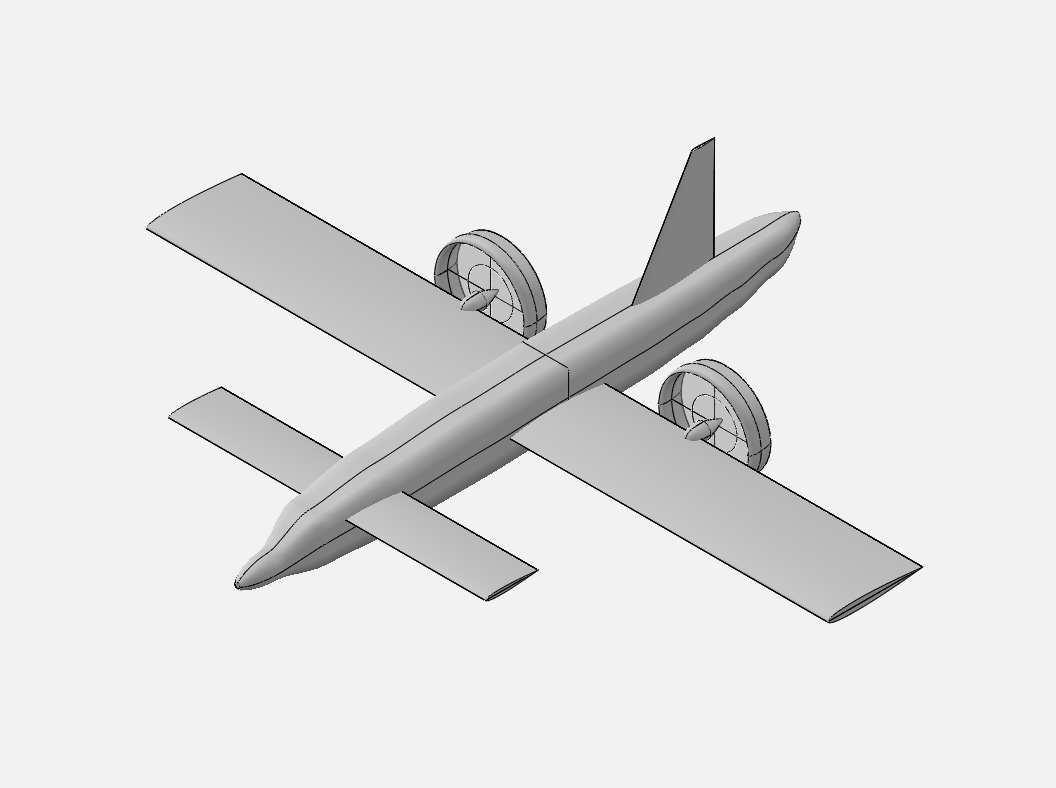
\includegraphics [scale = 0.7]{Figures/TitanLanderStraightWing.png}
    \caption{Second Iteration of the Titan Aircraft, with a Straight-Winged Variation of the Titan Lander}
    \label{fig:TitanLanderStraight}
\end{figure}



This third iteration included slight changes to the ducted fan sizing from the second. Additionally, the wing was changed from a standard delta wing to a double delta wing. The delta wing was placed higher on the z-axis of the fuselage, in order to maximize the hybrid wing-body element of the aircraft. Additionally this new configuration focused on proper tail sizing and the optimal tail configuration. The third design is shown below: 


 \begin{figure}[H]
 \centering 
    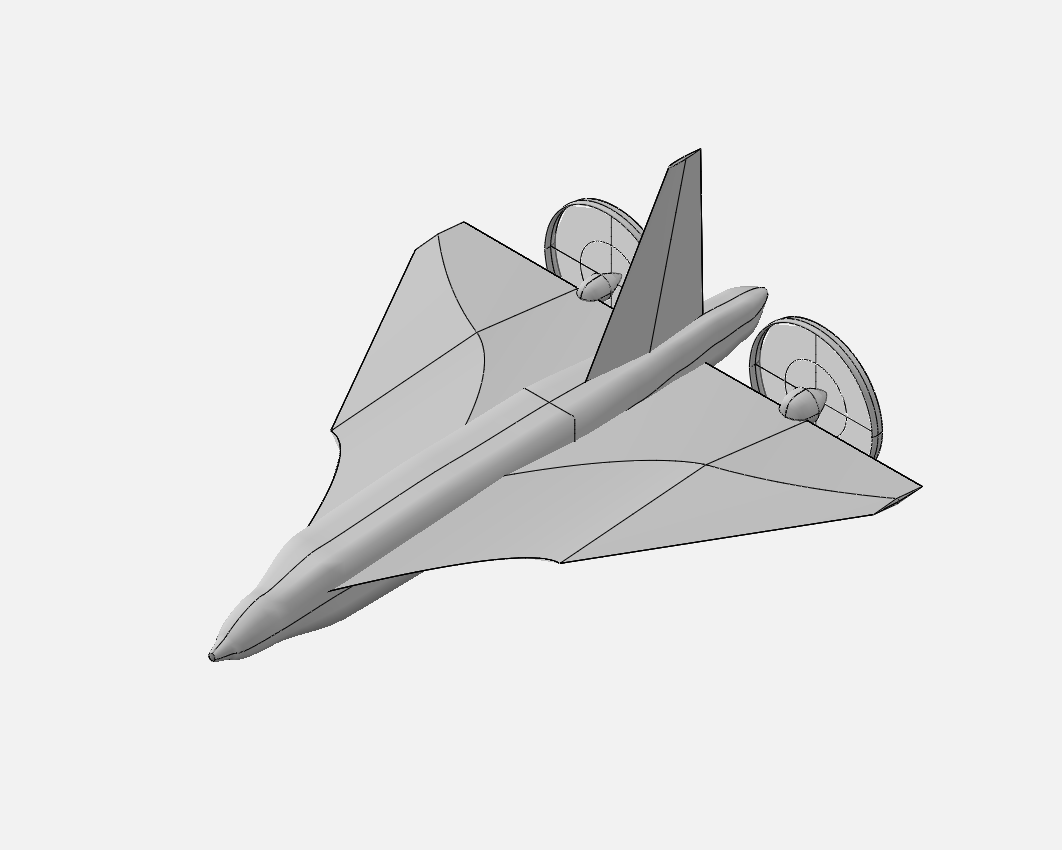
\includegraphics [scale = 0.7]{Figures/TitanLanderv2.png}
    \caption{Third Iteration of the Titan Aircraft, with a Double Delta Wing, and Larger Ducted Fans}
    \label{fig:TitanLanderv2}
\end{figure}

The fourth iteration was similar to the third, except a canard was added near the front of the fuselage to increase lift, as in the straight wing design. The main wing needed to compromise some of its area in order to account for the canard. This led to the main wing having an area of 1000 ${ft^{2}}$ and the canard having an area of 164 ${ft^{2}}$. The fourth iteration is shown below: 

\begin{figure}[H]
    \centering
    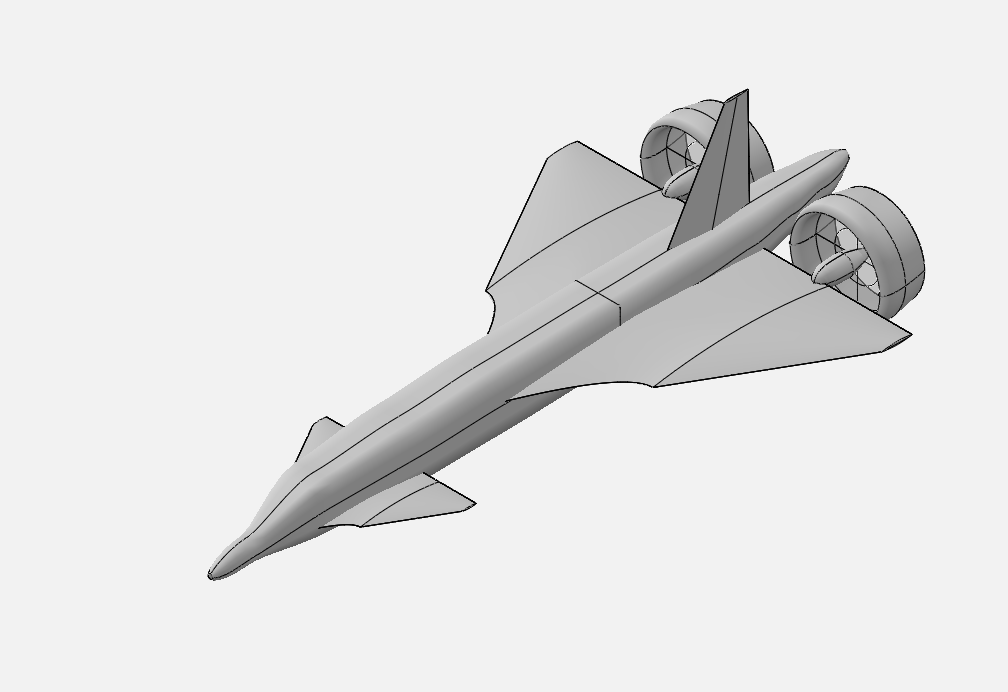
\includegraphics[width = 0.90\textwidth]{Figures/TitanLanderv6.png}
    \caption{Third Iteration of the Titan Aircraft, with a Canard}
    \label{fig:TitanLanderv6}
\end{figure}

The L/D value during cruise at an angle of attack of three was x, which is x compared to x. 

The fifth iteration utilized distributed electric propulsion, due to its many advantages, explained in the next section. The fifth iteration had four distributed fans that were sized as if they were distributed propellers. The fifth iteration also had a double delta wing with a biconvex airfoil. The fifth iteration if shown below: 

\begin{figure}[H]
    \centering
    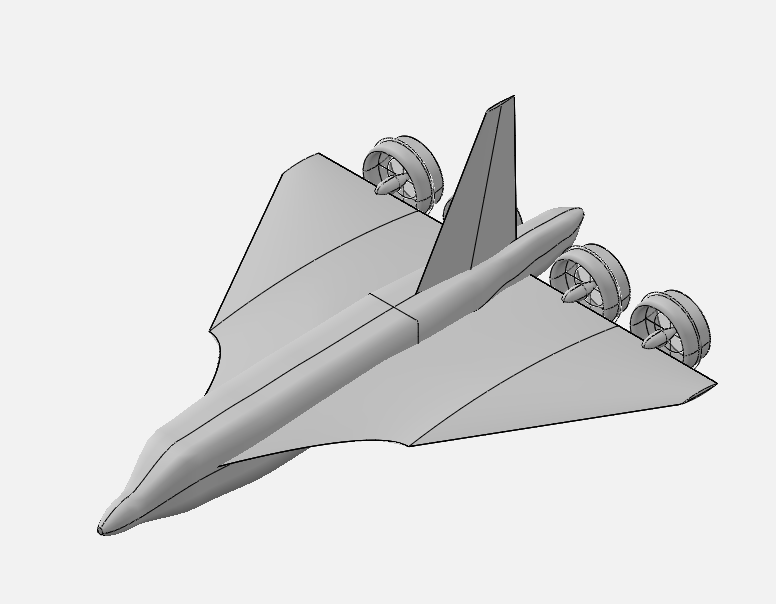
\includegraphics[width = 0.90\textwidth]{Figures/TitanLanderv7LeftIso.png}
    \caption{Fifth Iteration of the Titan Aircraft, with a Double Delta Wing and Four Distributed Ducted Fans}
    \label{fig:TitanLanderv7}
\end{figure}


The sixth iteration increased the number of distributed fans and included six ducted fans, sized as if they were propellers. The double delta wing was chosen with a biconvex airfoil. The final iteration is shown below: 

\begin{figure}[H]
    \centering
    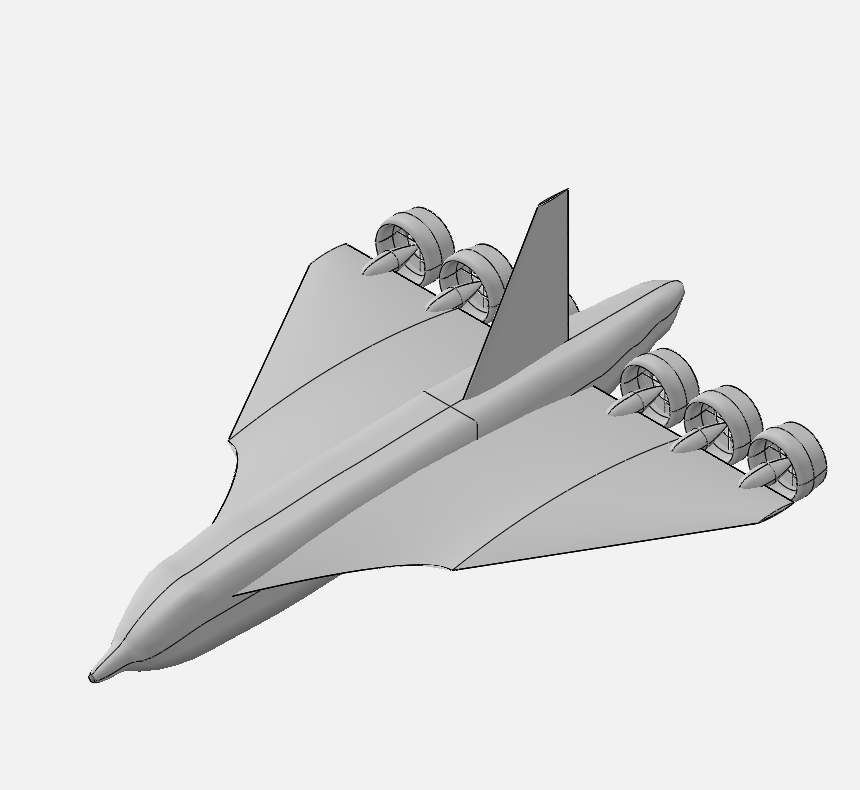
\includegraphics[width = 0.90\textwidth]{Figures/TitanLanderv11.png}
    \caption{Sixth Iteration of the Titan Aircraft, with a Double Delta Wing and Six Distributed Propellers}
    \label{fig:TitanLanderv11}
\end{figure}


The L/D value during cruise at an angle of attack of three was found to be x. This is x compared to x. The graph of L/D vs. angle of attack for Mach number 0.85 is shown below: 


The final model was similar to the sixth iteration, except a canard was added for increased lift, as described above with the fourth iteration. The final Titan Lander is shown below: 

\begin{figure}[H]
    \centering
    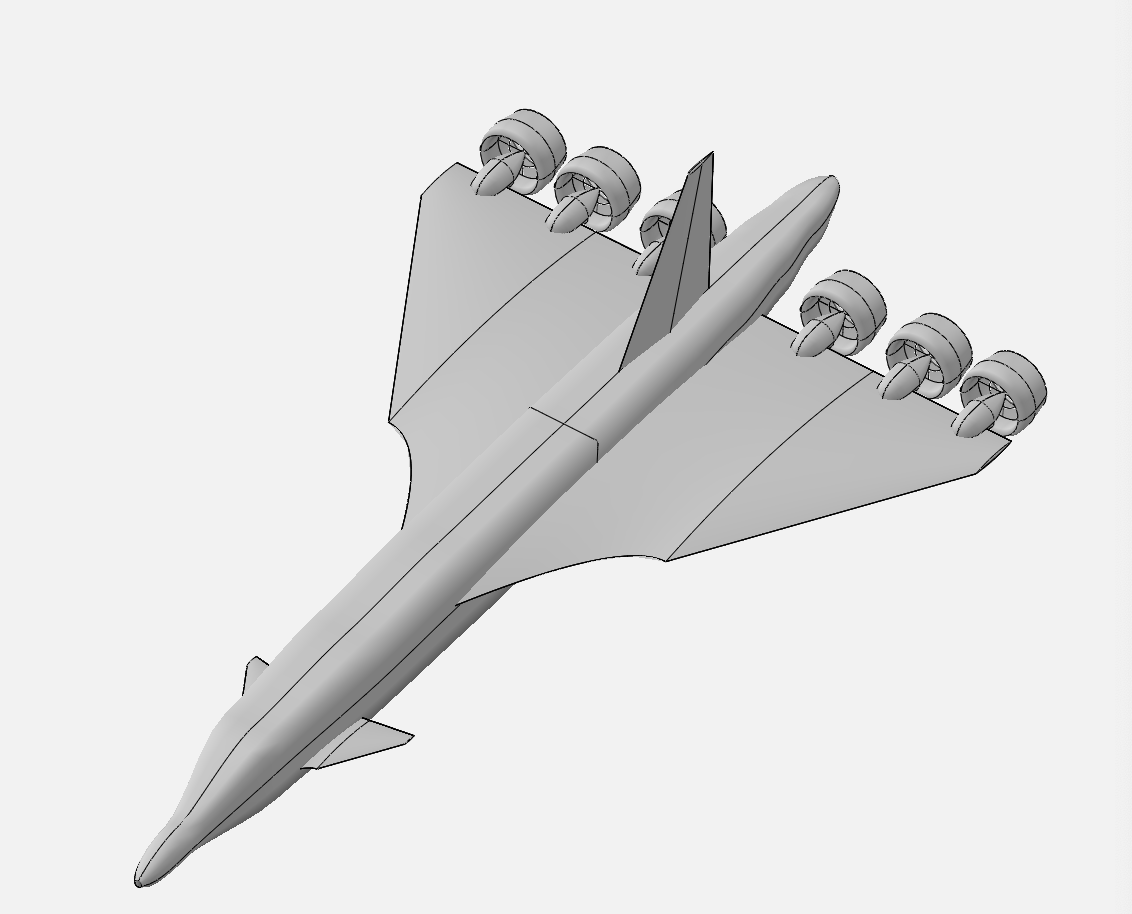
\includegraphics[width = 0.90\textwidth]{Figures/TitanLanderv13.png}
    \caption{Final Iteration of the Titan Aircraft, with a Double Delta Wing, Six Distributed Propellers, and a Canard}
    \label{fig:TitanLanderv13}
\end{figure}

\subsection{Tail Configuration and Sizing}
Since delta-winged aircrafts do not need horizontal stabilizers, it was decided that only a vertical tail (vertical stabilizer) was necessary. Every iteration utilized a delta wing in some way, so none of the designs have horizontal stabilizers. The tail is sized via the vertical tail volume coefficient ${C_{VT}}$, and its equation is shown below:

\begin{equation}
C_{VT} = \frac{L_{VT}*S_{VT}}{b_{w}*S_{w}}
\end {equation} 

where ${L_{VT}}$ is the moment arm of the vertical tail and is approximated as the distance from the tail quarter chord to the wing quarter-chord and ${S_{VT}}$ is the area of the vertical tail. Other delta-winged aircraft with vertical tails were investigated and used to estimate the vertical tail volume coefficient. ${C_{VT}}$ was found to be 0.07 [1]. Since ${b_{w}}$ and ${S_{w}}$ were found in the wing loading section, the tail area, ${S_{VT}}$, can be solved for. It was found to be 122.0707 ${ft^{2}}$.


\section{Flight Envelope}

For the final model, graphs of ${C_{l}}$, ${C_{d}}$, and ${C_{l}}/{C_{d}}$ versus Mach number were graphed in VSPAero and MATLAB in order to demonstrate performance. The Mach number demonstrates compressibility effects on the airflow [12]. Shock waves will be present above Mach 1 during hypersonic re-entry, so it is important to make sure the aircraft can still generate enough lift. The aircraft's performance over the entire flight envelope must be evaluated, in order to make sure it can operate during the various stages of flight: hypersonic entry, cruise, descent, landing and takeoff. The performance is measured through the aircraft's ${C_{l}}$ and ${C_{d}}$ values over the flight envelope. The critical performance graph for the final design are shown below: 

\begin{figure}[H]
    \centering
    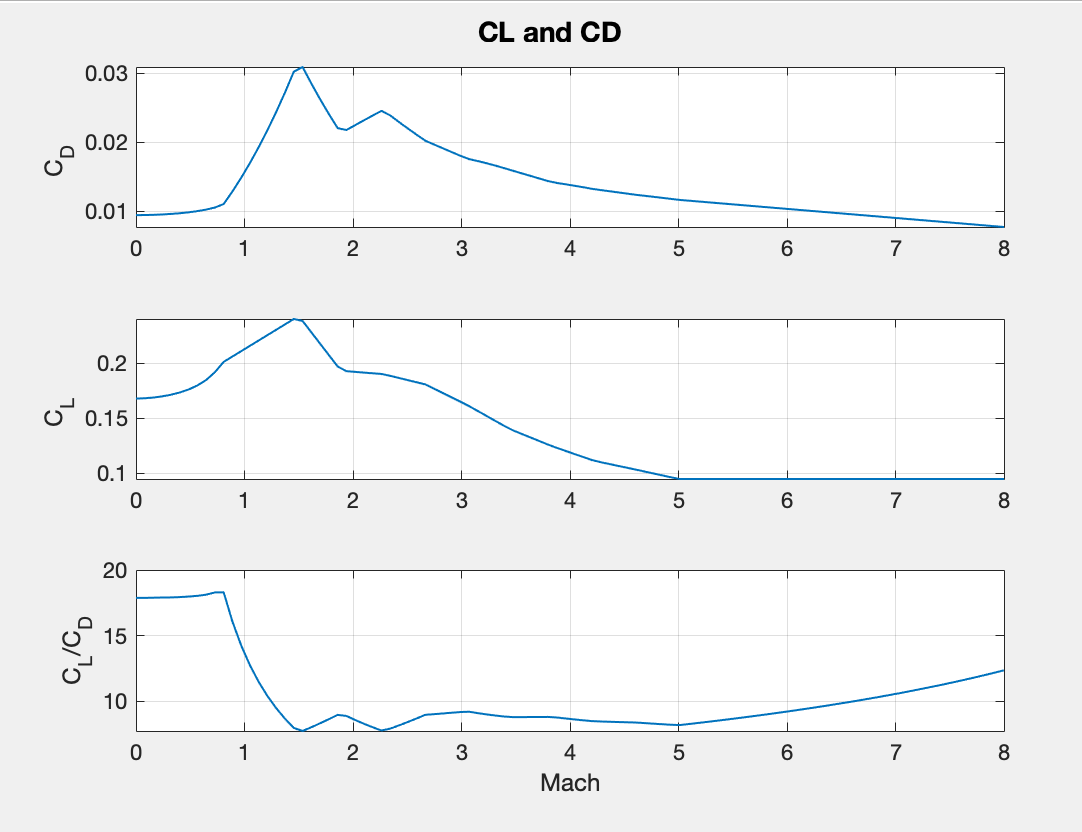
\includegraphics[width = 0.90\textwidth]{Figures/FlightEnvelope.png}
    \caption{${C_{l}}$, ${C_{d}}$, and ${C_{l}}/{C_{d}}$ versus Mach Number for the Final Titan Aircraft Design}
    \label{fig:FlightEnvelope}
\end{figure}

Additionally, graphs of ${C_{l}}$, ${C_{d}}$, and ${C_{l}}/{C_{d}}$ versus angle of attack were constructed in order to show how the aircraft responds to different pressure differentials between windward and leeward surfaces. The second critical performance graph is shown below: 

\begin{figure}[H]
    \centering
    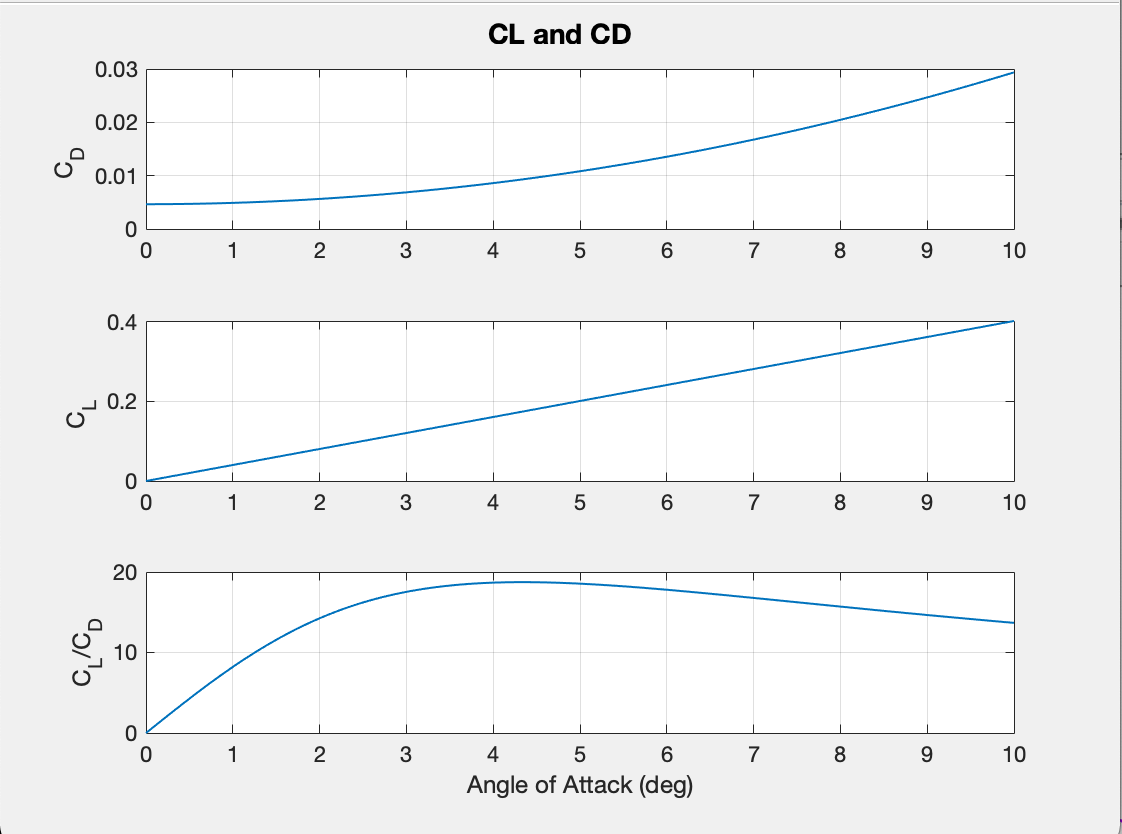
\includegraphics[width = 0.90\textwidth]{Figures/ClCdvAOA11.png}
    \caption{${C_{l}}$, ${C_{d}}$, and ${C_{l}}/{C_{d}}$ versus Angle of Attack for the Final Titan Aircraft Design}
    \label{fig:ClCdvAOA11}
\end{figure}

According to these graphs, the maximum value of ${C_{l}}/{C_{d}}$ is 18.74, occurring at an angle of attack 4.44. This is more than the initial estimate of ${L}/{D}$ in the thrust to wing loading graph during cruise, which was 18. 


The flight envelope can be compared to that of the previous iterations, in order to demonstrate improved performance with each design. Specifically, it is helpful to compare the ${C_{l}}/{C_{d}}$ values versus Mach for the different iterations. A graph of ${C_{l}}/{C_{d}}$ versus Mach for the sixth iteration compared to the final design is shown below: 

\begin{figure}[H]
    \centering
    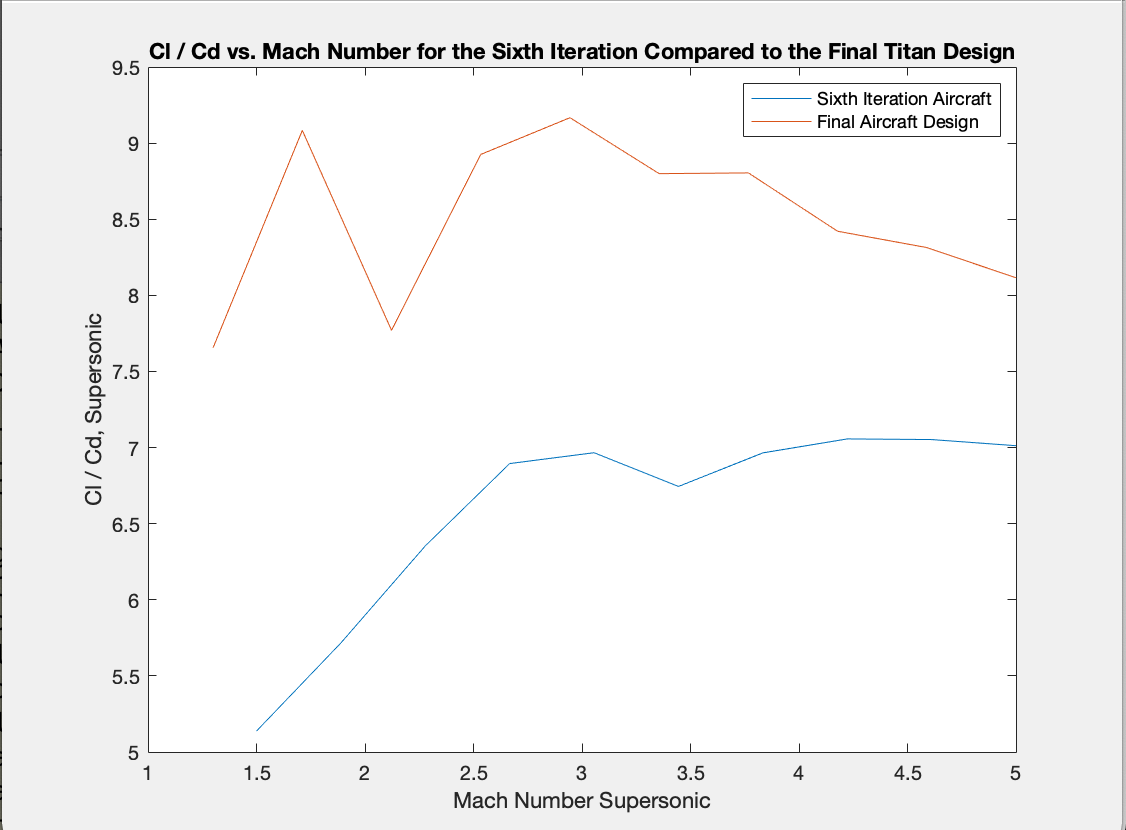
\includegraphics[width = 0.90\textwidth]{Figures/v11+v13Super.png}
    \caption{${C_{l}}$, ${C_{d}}$, and ${C_{l}}/{C_{d}}$ versus Mach Number for the Sixth Iteration Titan Aircraft Design}
    \label{fig:v11+v13Super}
\end{figure}

Clearly, the final aircraft design performs better than the sixth iteration at higher Mach numbers, which means better performance during re-entry into Titan's atmosphere. 



\section{Ducted Fan Sizing and Performance}
\label{sec:Ducted Fan Sizing and Performance}

\subsection{Introduction and Distributed Electric Propulsion}
\label{sec:Introduction and Distributed Electric Propulsion}

Ducted fans were chosen over propellers, since the duct enclosing the mechanical fan reduces thrust losses due to propeller tip speeds and increases the efficiency of the propeller [10]. Six distributed fans were chosen due to the many advantages of distributed electric propulsion systems. Distributed electric propulsion is a type of propulsion system where multiple electrically-driven propellers are connected to energy sources or power-generating devices [14]. Distributed electric propulsion offers the opportunity for more efficient propulsion and overall improved aircraft performance due to its many aero-propulsive coupling effects [14]. First, distributed electric propulsion can increase the boundary layer ingestion benefits described earlier in this chapter for improved propulsive efficiency [14]. Boundary layer ingestion can also lead to wake filling. Wake filling is used to help reduce energy losses from friction in the aircraft's trailing wake[15]. Additionally, the placement of the ducted fans can be used to mitigate the trailing vortices for increased lift [14].   


\subsection{Sizing}
The six ducted fans were sized as distributed propellers, therefore the speed-power coefficient was first calculated in order to size the fan. The speed power coefficient is defined by the equation: 

\begin{equation}
C_{s} = V_{cruise} * (\frac{\rho}{P*n^{2}})^{1/5}
\end{equation}

where n is the rotation speed of the fan and P is the power coming into the fan. The power coming into the fan is from the fusion engine, and each of the fans are to be connected in parallel to the main power source. Therefore, each fan has up to 1MW of power available to it. It was determined that only 0.5MW of power was needed to drive each fan, half of the total power available. A rotation speed of 4000RPM was estimated, based on similar engine data. Given these parameters, the speed power coefficient was found to be 2.0097. With the speed power coefficient, key parameters of each fan can be found using the NACA 640 charts, such as the advance ratio (J), fan efficiency, and the pitch of the fan. Estimating each fan as a propeller with a Clark Y airfoil and three blades, the chart used to find the advance ratio, efficiency, and pitch is shown below [9]: 
\begin{figure}[H]
 \centering 
    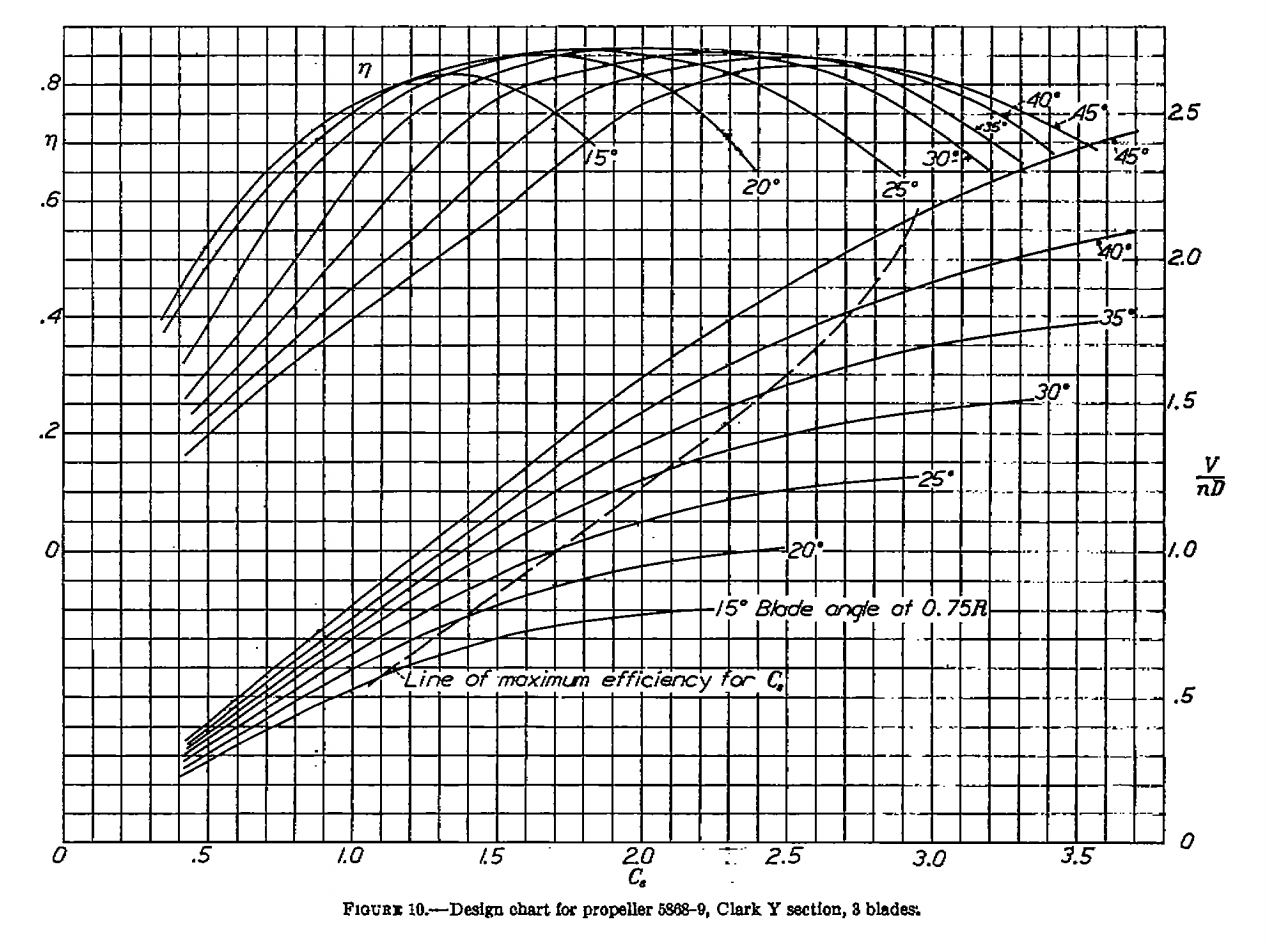
\includegraphics [width = 0.90\textwidth]{Figures/NACA.png}
    \caption{NACA 640 Chart Used to Size the Fans}
    \label{fig:NACA}
\end{figure}[H]
The advance ratio was found to be 0.8, therefore the blade angle at 0.75R, also known as the pitch, is 15 {\degree}. The efficiency of the fans is 0.82. The diameter of each fan is found with the formula: 

\begin{equation}
D =\frac{ V_{cruise}}{n*J}
\end{equation}
From this formula, the diameter of each propeller is around 5 ft. Adding a duct of the same diameter around each fan will increase the x, y, z. 

After finding the diameter, the coefficient of power and coefficient of thrust can be determined. The coefficient of power for the fan is found with the formula: 
\begin{equation}
C_{p} = \frac{P}{\rho*n^{3}*D^{5}}
\end{equation}

${C_{p}}$ was found to be 0.004. 

The coefficient of thrust is found with the formula: 
\begin{equation}
C_{T} = \frac{\eta* C_{p}}{J}
\end{equation}

The coefficient of thrust was found to be 0.996.

Finally, the thrust needed to power the fans is found through the formula: 

\begin{equation}
T = A_{fan}*N_{fans} * C_{t}
\end{equation}

where ${A_{fan}}$ is the area of each fan, and ${N_{fans}}$ is the total number of fans. The thrust required to power the fans was found to be 117.4 N. 


\subsubsection{Trailing Wakes and Optimal Number of Fans}

In order to determine the optimal number of ducted fans, the lift coefficient distribution needs to be analyzed for each DEP configuration. The ducted fans need to contribute to the aircraft's lift force, so the number of fans that provide the best lift for the aircraft without trailing wake interference will be the optimal number of fans. The Cl versus angel of attack graph for the final aircraft design was generated in the above section. Comparing it to the fifth iteration of the aircraft, which has four distributed fans, yields the following graph: 

\begin{figure}[H]
    \centering
    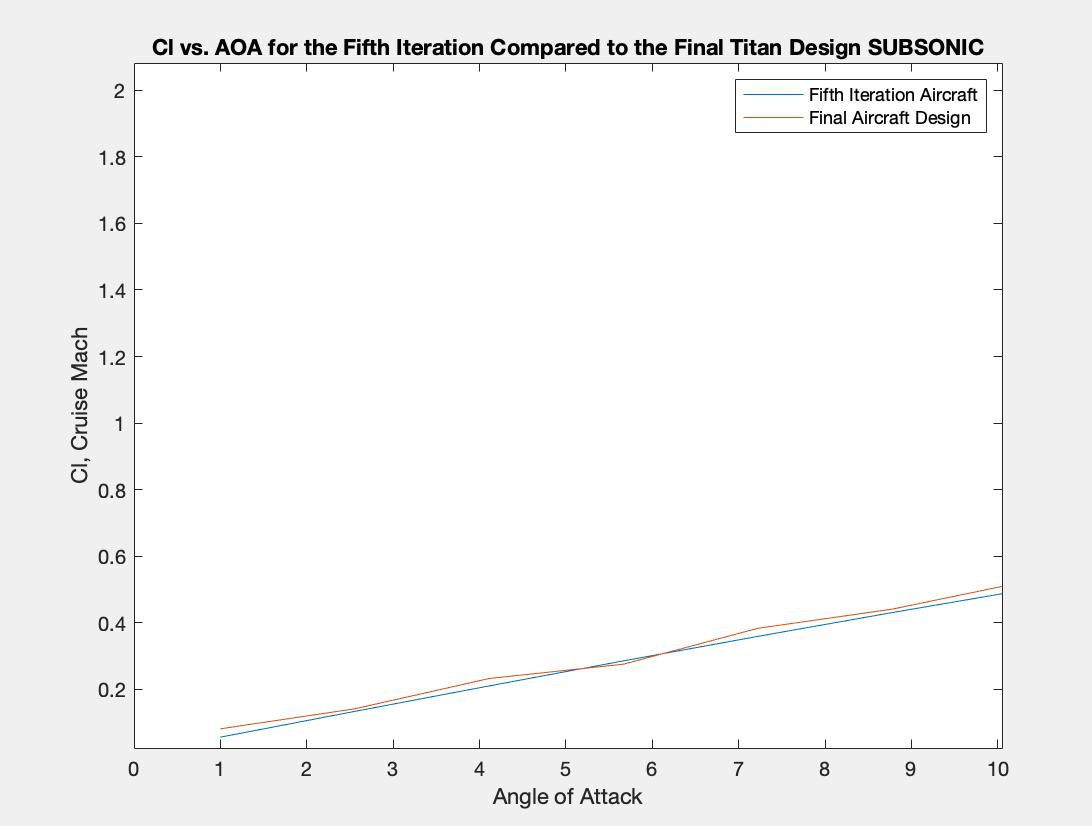
\includegraphics[width = 0.90\textwidth]{Figures/OptimalProp.png}
    \caption{${C_{l}}$ versus Angle of Attack Comparison between the Fifth Iteration and Final Design}
    \label{fig:OptimalProp}
\end{figure}

This graph shows that during transonic cruise, the six ducted fan configuration produces slightly more lift than the four ducted fan configuration, over a range of AOA from 0-10 ${\degree}$. Therefore, the six fan design is the better choice. 

The trailing wakes also need to be investigated when working with distributed propulsion. The trailing wakes for the final design are shown below: 
\begin{figure}[H]
    \centering
    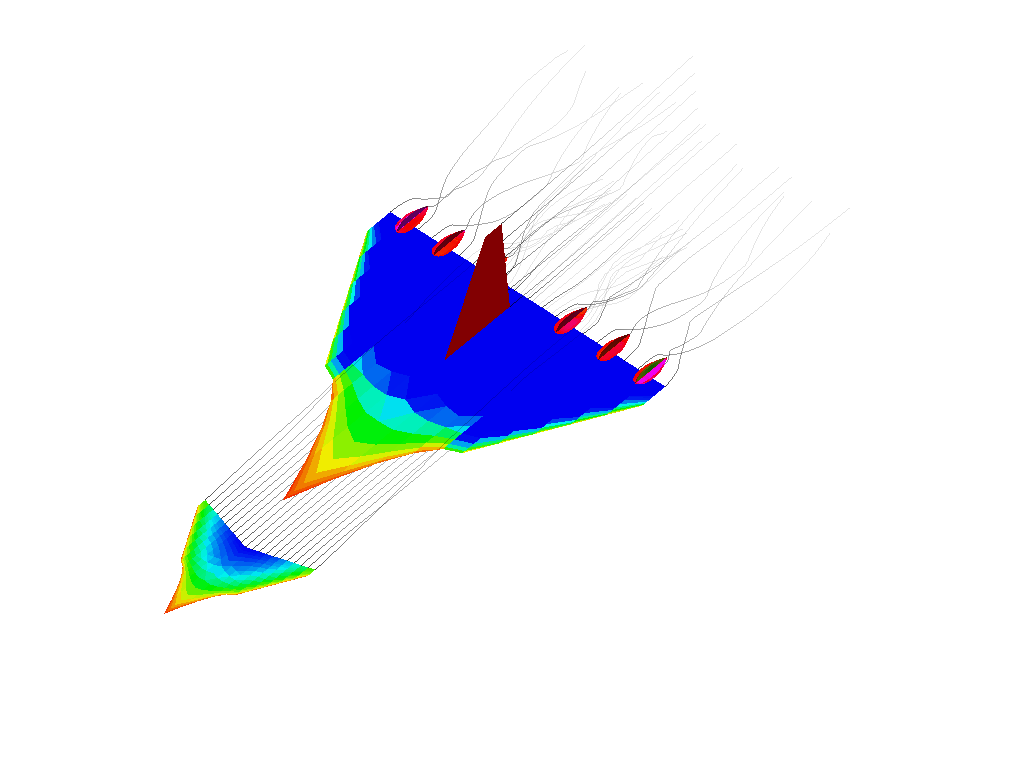
\includegraphics[width = 0.90\textwidth]{Figures/TrailingWakes.png}
    \caption{Trailing Wakes and Vorticity for the Final Design at Angle of Attack 4.11}
    \label{fig:TrailingWakes}
\end{figure}

As seen in Figure 15, strong vortices are forming over the wing, which will lead to increased lift during landing and takeof [12].
\end{document}






